%%%%%%%%%%%%%%%%%%%%%%%%%%%%%%%%%%%%%%%%%%%%%%
%                insertmeeting
% 1) Title (something creative & funny?)
% 2) Date (MM/DD/YYYY)
% 3) Location (ex. Hagerty High School)
% 4) People/Committees Present 
% 5) Picture 
% 6) Start Time & Stop Time (ex. 12:30AM to 4:30PM)
%%%%%%%%%%%%%%%%%%%%%%%%%%%%%%%%%%%%%%%%%%%%%%
\insertmeeting 
	{Kinematics Katastrophe} 
	{01/12/22} 
	{Hagerty High School}
	{Annika, Anouska, James, Nathan, Ritam, Samantha}
	{Images/RobotPics/robot.jpg}
	{2:30 - 4:30}
	
\hhscommittee{General}
\noindent\hfil\rule{\textwidth}{.4pt}\hfil
\subsubsection*{Goals}
\begin{itemize}
    \item Finish creating TricycleKinematics.kt and TricycleDrive.kt  

\end{itemize} 

\noindent\hfil\rule{\textwidth}{.4pt}\hfil

\subsubsection*{Accomplishments}
When we started testing our new methods today, we ran into a few issues. The first problem was that when we told the robot to go to a certain position, it often ended up going the correct direction, but it always moved to little or too much. This meant that our kinematic equations for calculating the desired robot heading were correct. The first section we began to troubleshoot was the x and y localization equations. Instead of telling the robot to move autonomously, we tried to turn on the robot but leave the unpowered wheels. This would allow us to check our calculations based purely on wheel rotations and encoder positions. We then logged the estimated position as we moved the robot around the field by hand. Surprisingly, the x and y coordinates were extremely accurate - only off by about a centimeter at most. This slight variation was expected, since our wheels were bound to slip during movement. The lack of dead wheel encoders due to our use of a single control hub meant that this problem could not be solved with conventional methods. We may have to continue testing the robot movement to see if this is a large enough problem to warrant a redesign. The next piece that we decided to check was how we sent information to the motors in our "SetDriveSignal" function. Upon further inspection, we realized that we made a mistake in one of the lines. One of the calculations for the needed motor power was using a method from "TankKinematics", not the new "TricycleKinematics". After fixing this quick fix, the robot moved correctly from one point to another. 

\begin{figure}[htp]
\centering
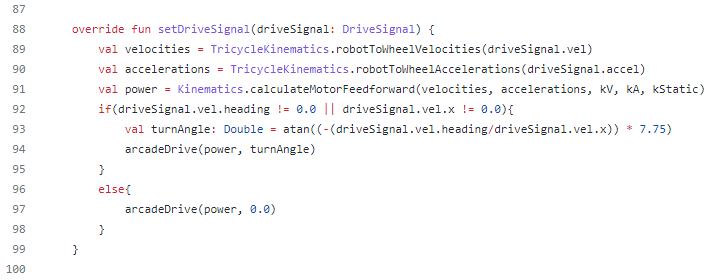
\includegraphics[width=0.95\textwidth, angle=0]{Meetings/January/01-12-22/1.12.22 drivesignal - James Hu.PNG}
\caption{Our modified driveSignal class that fixed the robot's incorrect movement}
\label{fig:011222_1}
\end{figure}

\whatsnext{
\begin{itemize}
    \item Begin to integrate our new Road Runner Tricycle foundation into a TRC-event capable drivebase.
\end{itemize} 
}

